% 原文PDF112--123頁（本文90--101頁）、3.4--3.5。
\subsectionlink{Weyl 異常}\label{sec:3.4}

弦理論の重要な特徴は、すべての時空背景で整合的なのではなく、ある条件を満たす背景でのみ整合的であるという点である。平坦な時空におけるボソン弦理論では、その条件は $D=26$ である。これは最初、散乱振幅の病的な振る舞いとして発見された。光円錐による解析では、1.3節で手短に、かなり直観的に説明したように、Lorentz 不変性の喪失として現れる。この制限の根本的な原因は、世界面の局所対称性における異常である。現在の形式では、その異常は Weyl 対称性にある。$T^a{}_a$ は古典的にはゼロだが、量子論ではそうではない。

場の量子論を学んだ読者は、同じ言葉では説明されなかったかもしれないが、すでに関連する異常に出会っている。大域的な Weyl 変換、すなわち $\omega(\sigma)=\text{定数}$ は、長さ全体のスケール変換と等価である。四次元における、よく知られたいくつかの場の理論は、そのようなスケール変換の下で古典的に不変である。これには、$\phi^4$ 相互作用をもつ質量のないスカラー場の理論や、非 Abel ゲージ理論が含まれる。Lagrangian に次元をもつパラメータが含まれず、どの場合も結合定数は無次元なので、スケール不変性は明らかである。しかし、量子論の発散により、それぞれの理論にゼロでない繰り込み群のベータ関数があることを、われわれは知っている。これは、有効結合定数が実際には長さの尺度の関数であることを意味する。対応して、エネルギー運動量テンソルのトレースは古典論ではゼロであるが、量子効果を考慮するとゼロでなくなり、ベータ関数に比例する。

前節では、異常の可能性を無視した。この点を確かめる必要がある。ゲージ固定した経路積分 $Z[g]$ は、本当に基準計量の選択に依存しないのだろうか。
\begin{equation}
Z[g^\zeta]=Z[g]\;?
\tag{3.4.1}\label{eq:3.4.1}
\end{equation}
4.2節では、これをより一般的なゲージの変更へ拡張する。便宜上、以下では $g$ のハットを省く。また、追加の挿入を含む経路積分
\begin{equation}
\langle\cdots\rangle_g
\equiv\int[dX\,db\,dc]\,\exp\bigl(-S[X,b,c,g]\bigr)\cdots
\tag{3.4.2}\label{eq:3.4.2}
\end{equation}
にも関心がある。その場合には、
\begin{equation}
\langle\cdots\rangle_{g^\zeta}=\langle\cdots\rangle_g
\tag{3.4.3}\label{eq:3.4.3}
\end{equation}
も要求する。現時点では、挿入そのものの詳細には関心がない。それは次の二つの節の主題となる。そこで、「$\cdots$」に含まれる場の位置の近傍でゼロとなるゲージ変換 $\zeta$ に注意を限る。つまり、演算子方程式として Weyl 不変性が成り立つことを要求している。

量子論で微分同相不変性と Poincaré 不変性を保つのは容易である。たとえば、A.1節で調和振動子について行ったように、Pauli--Villars レギュレータを用い、質量をもつレギュレータ場の経路積分で割ることによって、ゲージ固定した経路積分を定義できる。質量をもつレギュレータ場は、微分同相不変かつ Poincaré 不変な仕方で計量に結合できる。しかし、レギュレータ場 $Y^\mu$ の、微分同相不変かつ Poincaré 不変な質量項 $\mu^2\int d^2\sigma\,g^{1/2}Y^\mu Y_\mu$ は、Weyl 不変ではない。したがって、Weyl 不変性は直接確かめねばならない。Weyl 変換に対して不変性\hyperref[eq:3.4.3]{(3.4.3)}は成り立つだろうか。任意の Weyl 変換は、無限小変換を繰り返した結果として得られるため、後者を調べれば十分である。

エネルギー運動量テンソル $T^{ab}$ は、計量に関する経路積分の無限小変分である。
\begin{equation}
\delta\langle\cdots\rangle_g
=-\frac1{4\pi}\int d^2\sigma\,g(\sigma)^{1/2}
\delta g_{ab}(\sigma)\left\langle T^{ab}(\sigma)\cdots\right\rangle_g.
\tag{3.4.4}\label{eq:3.4.4}
\end{equation}
古典的には、$T^{ab}$ はすべて作用の変分から生じ、これは Noether の定義
\begin{equation}
T^{ab}(\sigma)\overset{\text{古典的}}{=}
\frac{4\pi}{g(\sigma)^{1/2}}
\frac{\delta}{\delta g_{ab}(\sigma)}S
\tag{3.4.5}\label{eq:3.4.5}
\end{equation}
と一致する。また、平坦な世界面の極限では、それまでの定義に帰着する。$\delta g_{ab}$ を座標変換の形にとれば、経路積分の微分同相不変性は $T^{ab}$ の保存を意味する。

以下の解析では、まず境界項の可能性を無視する。Weyl 変換に対して、$T^{ab}$ の定義\hyperref[eq:3.4.4]{(3.4.4)}は
\begin{equation}
\delta_{\mathrm W}\langle\cdots\rangle_g
=-\frac1{2\pi}\int d^2\sigma\,g(\sigma)^{1/2}
\delta\omega(\sigma)\left\langle T^a{}_a(\sigma)\cdots\right\rangle_g
\tag{3.4.6}\label{eq:3.4.6}
\end{equation}
を意味する。したがって、一般の挿入「$\cdots$」を含む場合の Weyl 不変性は、エネルギー運動量テンソルのトレースがゼロであるという演算子としての主張に言い換えられる。
\begin{equation}
T^a{}_a\overset{?}{=}0.
\tag{3.4.7}\label{eq:3.4.7}
\end{equation}
古典作用は Weyl 不変であるが、完全にゲージ不変なレギュレータを見いだせていないため、量子論ではトレースがゼロでないかもしれない。微分同相不変性と Poincaré 不変性は保っているので、トレースはそれらに対して不変でなければならない。また、平坦な場合の理論が共形不変であることを前章から知っているので、平坦な場合にはゼロにならねばならない。すると可能性は一つしか残らない。
\begin{equation}
T^a{}_a=a_1R.
\tag{3.4.8}\label{eq:3.4.8}
\end{equation}
ここで $a_1$ はある定数であり、$R$ はやはり世界面の Ricci スカラーである。二つを超える微分を含む項は、次元の理由から禁じられる。世界面の長さを単位として測ると、$g_{ab}$ と $X^\mu$ はともに無次元なので、式\hyperref[eq:3.4.8]{(3.4.8)}の定数 $a_1$ も無次元である。より多くの微分を含む項の係数は、経路積分の定義に用いたカットオフ長さの正のべきを含むことになる。したがって、カットオフをゼロにする極限で、そのような項は消える。

\subsubsection*{Weyl 異常の計算}

ゲージ不変な理論を妨げうるものは、一つの数 $a_1$ に帰着した。実際、この数は、すでに計算した量、すなわち平坦な世界面上の CFT の中心電荷 $c$ に比例する。$a_1$ と $c$ はどちらも、成分は異なるものの、エネルギー運動量テンソルの二点関数に関係している。両者の正確な関係を得るには、次のように微分同相不変性を用いる必要がある。

共形ゲージでは、
\begin{equation}
T_{z\bar z}=\frac{a_1}2g_{z\bar z}R.
\tag{3.4.9}\label{eq:3.4.9}
\end{equation}
共変微分をとると、
\begin{equation}
\nabla^{\bar z}T_{\bar z z}
=\frac{a_1}2\nabla^{\bar z}(g_{z\bar z}R)
=\frac{a_1}2\partial_zR.
\tag{3.4.10}\label{eq:3.4.10}
\end{equation}
ここでは、計量が共変的に一定であることを用いた。すると、$T_{ab}$ の保存則から、
\begin{equation}
\nabla^zT_{zz}=-\nabla^{\bar z}T_{\bar z z}
=-\frac{a_1}2\partial_zR.
\tag{3.4.11}\label{eq:3.4.11}
\end{equation}
$a_1$ を決めるため、左辺と右辺の Weyl 変換を比較する。右辺の Weyl 変換(3.3.5)は
\begin{equation}
a_1\partial_z\nabla^2\delta\omega
\approx4a_1\partial_z^2\partial_{\bar z}\delta\omega
\tag{3.4.12}\label{eq:3.4.12}
\end{equation}
である。ここでは、平坦な世界面の周りで展開した。$T_{zz}$ の Weyl 変換を得るには、まず共形変換\hyperref[eq:2.4.24]{(2.4.24)}を用いる。
\begin{equation}
\epsilon^{-1}\delta T_{zz}(z)
=-\frac c{12}\partial_z^3v^z(z)
-2\partial_zv^z(z)T_{zz}(z)-v^z(z)\partial_zT_{zz}(z).
\tag{3.4.13}\label{eq:3.4.13}
\end{equation}
3.3節の議論によると、この共形変換は座標変換 $\delta z=\epsilon v$ と、Weyl 変換 $2\delta\omega=\epsilon\partial v+\epsilon(\partial v)^*$ からなる。変分の最後の二項はテンソルの座標変換である。したがって、平坦な空間の周りの最低次における Weyl 変換は
\begin{equation}
\delta_{\mathrm W}T_{zz}=-\frac c6\partial_z^2\delta\omega
\tag{3.4.14}\label{eq:3.4.14}
\end{equation}
である。$\partial^z=2\partial_{\bar z}$ を作用させ、変換\hyperref[eq:3.4.12]{(3.4.12)}と比較すると、
\begin{equation}
c=-12a_1,\qquad T^a{}_a=-\frac c{12}R
\tag{3.4.15}\label{eq:3.4.15}
\end{equation}
を得る。

これを、少し長い別の道筋でもう一度導こう。その途中で、有用な中間結果が得られる。共形ゲージでは、
\begin{align}
R&=-2\exp(-2\omega)\partial_a\partial_a\omega,
\tag{3.4.16a}\label{eq:3.4.16a}\\
\nabla^2&=\exp(-2\omega)\partial_a\partial_a.
\tag{3.4.16b}\label{eq:3.4.16b}
\end{align}
二つの下付き添字による縮約は、$\delta^{ab}\partial_a\partial_b$ を意味する。$Z[g]$ の Weyl 変分\hyperref[eq:3.4.6]{(3.4.6)}は
\begin{equation}
\delta_{\mathrm W}Z[\exp(2\omega)\delta]
=\frac{a_1}{\pi}Z[\exp(2\omega)\delta]
\int d^2\sigma\,\delta\omega\,\partial_a\partial_a\omega
\tag{3.4.17}\label{eq:3.4.17}
\end{equation}
となる。ここで「$\exp(2\omega)\delta$」は共形ゲージを表す。これは直ちに積分でき、
\begin{equation}
Z[\exp(2\omega)\delta]
=Z[\delta]\exp\left(-\frac{a_1}{2\pi}
\int d^2\sigma\,\partial_a\omega\partial_a\omega\right)
\tag{3.4.18}\label{eq:3.4.18}
\end{equation}
となる。すべての計量は共形計量と微分同相変換で等価なので、式\hyperref[eq:3.4.18]{(3.4.18)}は、実際には $Z[g]$ の計量依存性を完全に決めている。共形ゲージで式\hyperref[eq:3.4.18]{(3.4.18)}に帰着する、微分同相不変な表式を見つければよい。関係式\hyperref[eq:3.4.16a]{(3.4.16)}を用いると、求める表式が
\begin{equation}
Z[g]=Z[\delta]\exp\left[
\frac{a_1}{8\pi}\int d^2\sigma\int d^2\sigma'\,
g^{1/2}R(\sigma)G(\sigma,\sigma')g^{1/2}R(\sigma')
\right]
\tag{3.4.19}\label{eq:3.4.19}
\end{equation}
であることを確認できる。ただし、スカラーの Green 関数は
\begin{equation}
g(\sigma)^{1/2}\nabla^2G(\sigma,\sigma')
=\delta^2(\sigma-\sigma')
\tag{3.4.20}\label{eq:3.4.20}
\end{equation}
によって定義される。これは興味深い結果である。経路積分が、異常の方程式によって完全に決まっている。

次に、平坦な背景の周りで $Z[g]$ を展開し、$g_{ab}=\delta_{ab}+h_{ab}$ とおいて、$h_{\bar z\bar z}$ の二次の項を残す。Ricci スカラーは $h_{\bar z\bar z}$ の一次では $4\partial_z^2h_{\bar z\bar z}$ なので、$z=z'$ の接触項を無視すると、
\begin{equation}
\begin{aligned}
\ln\frac{Z[\delta+h]}{Z[\delta]}
&\approx\frac{a_1}{8\pi^2}
\int d^2z\int d^2z'\,
\bigl(\partial_z^2\ln|z-z'|^2\bigr)\\
&\qquad{}\times
h_{\bar z\bar z}(z,\bar z)\partial_{z'}^2h_{\bar z\bar z}(z',\bar z')\\
&=-\frac{3a_1}{4\pi^2}
\int d^2z\int d^2z'\,
\frac{h_{\bar z\bar z}(z,\bar z)h_{\bar z\bar z}(z',\bar z')}
{(z-z')^4}.
\end{aligned}
\tag{3.4.21}\label{eq:3.4.21}
\end{equation}
これは、計量についての二次の摂動論によっても計算できる。式\hyperref[eq:3.4.4]{(3.4.4)}より、
\begin{equation}
\begin{aligned}
\ln\frac{Z[\delta+h]}{Z[\delta]}
&\approx\frac1{8\pi^2}
\int d^2z\int d^2z'\,
h_{\bar z\bar z}(z,\bar z)h_{\bar z\bar z}(z',\bar z')\\
&\qquad{}\times
\left\langle T_{zz}(z)T_{zz}(z')\right\rangle_\delta
\end{aligned}
\tag{3.4.22}\label{eq:3.4.22}
\end{equation}
となる。ここで標準的な $TT$ の OPE \hyperref[eq:2.4.25]{(2.4.25)}を用いる。最初の項以外はすべてゼロでないスピンをもつ演算子を含むので、回転不変性によって消え、
$\langle T_{zz}(z)T_{zz}(z')\rangle_\delta=\tfrac12c(z-z')^{-4}$
が残る。Weyl 異常から得られた結果\hyperref[eq:3.4.21]{(3.4.21)}と比較すると、再び式\hyperref[eq:3.4.15]{(3.4.15)}が得られる。

\subsubsection*{考察}

世界面の理論は、中心電荷 $D$ をもつ $X^\mu$ と、$\lambda=2$ では中心電荷\hyperref[eq:2.5.12]{(2.5.12)}が $-26$ となるゴーストからなる。したがって、
\begin{equation}
c=c^X+c^g=D-26.
\tag{3.4.23}\label{eq:3.4.23}
\end{equation}
この理論が Weyl 不変となるのは $D=26$ の場合だけであり、第1章で見いだした Lorentz 不変性の条件と同じである。Weyl 異常がゼロでないとき、異なるゲージの選択は等価でなく、異常をもつゲージ理論と同様に、どの選択も共変性の喪失やユニタリティの喪失といった病的な性質をもたらす。たとえば光円錐ゲージでは、時空軸を違うものに選ぶにはゲージの変更が必要である。そのため、根底にある Weyl 異常が Lorentz 異常として現れる。

もう一つ試みうることがある。Weyl 不変性を無視し、微分同相不変性だけをゲージ対称性として扱うのである。すると計量は、一つの実自由度 $\omega(\sigma)$ をもち、これはゲージ固定されるのではなく積分されることになる。これはとくにもっともらしい。式\hyperref[eq:3.4.18]{(3.4.18)}の量子効果は、$X^\mu$ の一つの作用とよく似た $\omega$ の作用を生成しており、$D<26$ ではその符号が空間的な次元の符号になるからである。しかし、$\omega$ の微分同相変換、したがってそのエネルギー運動量テンソルが $X^\mu$ のものと異なるため、物理は少し変わったものになる。実際、この理論は線形ディラトン CFT である。したがって $(D+1)$ 次元の Lorentz 不変性はなく、宇宙のうちわれわれがいる領域の物理を理解するという当面の目的には、この理論は役に立たない。しかし興味深い模型であり、9.9節でこの点に簡単に立ち戻る。

上で、平坦な世界面の CFT が、Weyl 不変な仕方で曲がった計量に結合できるための必要十分条件は、全中心電荷 $c$ がゼロであることだとわかった。しかし、ここには逆説がある。同じ議論は反正則な中心電荷 $\tilde c$ にも適用できるが、$bc$ CFT の例で見たように、$c$ と $\tilde c$ は等しいとは限らない。要点は、式\hyperref[eq:3.4.11]{(3.4.11)}と\hyperref[eq:3.4.19]{(3.4.19)}で、世界面の微分同相不変性を暗黙のうちに仮定していたことである。$c\ne\tilde c$ なら、$O(h_{zz}^2)$ と $O(h_{\bar z\bar z}^2)$ の両方の計算と一致する微分同相不変な表式は存在しない。この場合、その CFT を微分同相不変な仕方で曲がった計量に結合することはできない。微分同相異常、すなわち重力異常があるのである。この逆説は、CFT が重力異常をもたないためには $c=\tilde c$ が必要であることを示す。また、この条件が十分であることも示せる。

\subsubsection*{境界を含む場合}

まず式\hyperref[eq:3.4.8]{(3.4.8)}に戻り、より一般的な可能性
\begin{equation}
T^a{}_a=a_1R+a_2
\tag{3.4.24}\label{eq:3.4.24}
\end{equation}
を考えよう。これは微分同相不変性によって許されるが、平坦な極限でゼロにならない。先には、式\hyperref[eq:2.3.15b]{(2.3.15b)}の下の脚注で説明したように、その $T_{ab}$ の選び方によって $a_2$ をゼロにした。等価的にいえば、平坦な世界面上に複数の保存する $T_{ab}$ が存在するということは、曲がった計量への結合の仕方にいくらか自由があることを意味する。とくに、作用には
\begin{equation}
S_{\mathrm{ct}}=b\int d^2\sigma\,g^{1/2}
\tag{3.4.25}\label{eq:3.4.25}
\end{equation}
を加えられる。これは二次元の宇宙定数であり、Weyl 不変ではない。これを加えると $T_{ab}$ に $2\pi b g_{ab}$ が加わるため、トレース\hyperref[eq:3.4.24]{(3.4.24)}は
\begin{equation}
T^a{}_a=a_1R+(a_2+4\pi b)
\tag{3.4.26}\label{eq:3.4.26}
\end{equation}
となる。したがって、$b=-a_2/4\pi$ とおくことで第2項を消せる。これが、式\hyperref[eq:2.3.15b]{(2.3.15b)}で暗黙のうちに行ったことである。$a_2$ と $b$ の個別の値は定義に依存し、興味の対象ではない。

そのような局所的な相殺項によって $a_1$ を除くことはできない。たとえば、すでに述べたように、$\int d^2\sigma\,g^{1/2}R$ は Weyl 不変である。したがって、$a_1$ がゼロでなければ、Weyl 対称性には実際に異常がある。

次に境界の効果を考える。境界項を含めると、可能な最も一般的な変分は次である。\footnote[3]{すべての項は、場 $X^\mu$ に依存しないことを要求する。自由場の理論では、これが成り立つことを示せる。3.7節で相互作用する場合を考えるときには、Weyl 異常はより一般的な形をとる。}
\begin{equation}
\begin{aligned}
\delta_{\mathrm W}\ln\langle\cdots\rangle_g
={}&-\frac1{2\pi}\int_Md^2\sigma\,g^{1/2}(a_1R+a_2)\delta\omega\\
&-\frac1{2\pi}\int_{\partial M}ds\,
(a_3+a_4k+a_5n^a\partial_a)\delta\omega.
\end{aligned}
\tag{3.4.27}\label{eq:3.4.27}
\end{equation}
ここで、やはり $k=-t^an_b\nabla_at^b$ は境界の測地曲率である。可能な相殺項は
\begin{equation}
S_{\mathrm{ct}}=\int_Md^2\sigma\,g^{1/2}b_1
+\int_{\partial M}ds\,(b_2+b_3k)
\tag{3.4.28}\label{eq:3.4.28}
\end{equation}
である。$b_3$ の項は、式(3.2.3b)の Euler 数に含まれる測地曲率の項に追加されるものである。$ds$ と単位ベクトル $t,n$ の計量依存性も忘れずに含めると、$S_{\mathrm{ct}}$ の Weyl 変分は
\begin{equation}
\delta_{\mathrm W}S_{\mathrm{ct}}
=2\int_Md^2\sigma\,g^{1/2}b_1\delta\omega
+\int_{\partial M}ds\,(b_2+b_3n^a\partial_a)\delta\omega
\tag{3.4.29}\label{eq:3.4.29}
\end{equation}
となる。$b_1,b_2,b_3$ を選ぶことで $a_2,a_3,a_5$ をゼロにでき、異常の候補として $a_1,a_4$ が残ることがわかる。もう一つ使える道具がある。Wess--Zumino の整合性条件である。二階の汎関数変分をとると、
\begin{equation}
\begin{aligned}
&\delta_{\mathrm W_1}\bigl(\delta_{\mathrm W_2}\ln\langle\cdots\rangle_g\bigr)\\
&\quad=\frac{a_1}{\pi}\int_Md^2\sigma\,g^{1/2}
\delta\omega_2\nabla^2\delta\omega_1
-\frac{a_4}{2\pi}\int_{\partial M}ds\,
\delta\omega_2n^a\partial_a\delta\omega_1\\
&\quad=-\frac{a_1}{\pi}\int_Md^2\sigma\,g^{1/2}
\partial_a\delta\omega_2\partial^a\delta\omega_1
+\frac{2a_1-a_4}{2\pi}\int_{\partial M}ds\,
n^a\delta\omega_2\partial_a\delta\omega_1.
\end{aligned}
\tag{3.4.30}\label{eq:3.4.30}
\end{equation}
これは二階の（汎関数）微分なので、定義により $\delta\omega_1,\delta\omega_2$ に関して対称でなければならない。第1項は対称だが、第2項は対称でないので、$a_4=2a_1$ となる。したがって、開弦の境界条件を課した境界は、新たな Weyl 異常を生じさせない。量子論で Weyl 不変性が成り立つための必要十分条件は、$a_1=-c/12$ がゼロになることである。これは、世界面の内部の局所的な物理によって決まる。

Wess--Zumino の整合性条件は、可能な異常の形に非常に強い制限を課す。第二の応用として、中心電荷が定数であることを示せる。上では Lorentz 不変性と次元解析からこれが従ったが、より一般的な CFT では、
\begin{equation}
T^a{}_a(\sigma)=-\frac{\mathcal C(\sigma)}{12}R(\sigma)
\tag{3.4.31}\label{eq:3.4.31}
\end{equation}
のようになることも考えられる。ここで $\mathcal C(\sigma)$ は、ある局所演算子である。とくに、平坦な世界面ではトレースは依然としてゼロになる。$a_1$ の代わりに $-\mathcal C(\sigma)/12$ を用いて計算\hyperref[eq:3.4.30]{(3.4.30)}を繰り返すと、部分積分から、$\partial_a\mathcal C(\sigma)$ に比例する追加の非対称な項が生じる。したがって、整合性条件は、$\mathcal C(\sigma)$ を含む期待値が位置に依存しないことを意味する。これは、$\mathcal C(\sigma)$ 自身が単なる数値定数 $c$ であることを意味する。

\subsectionlink{散乱振幅}\label{sec:3.5}

与えられた始状態と終状態の曲線を境界にもつ、すべての世界面について和をとるという考えは、自然に思える。しかし、これを世界面の局所対称性と両立するように定義するのは難しく、得られる振幅もかなり複雑である。振幅が簡単になる特殊な場合が一つある。弦の源を無限遠へ持っていく極限である。これは、入射する弦と出ていく弦を指定した散乱振幅、すなわち $S$ 行列要素に対応する。本書の大部分では、$S$ 行列と、それに類する「オンシェル」の問題に範囲を限る。漸近的な過程だけでなく、有限の時刻における系の状態も議論できるようにしたいので、これは完全に満足のいくものではない。当面は $S$ 行列に注目する。それはよく理解されている一方、オフシェルの弦理論をどのように考えるのが正しいかは明らかでないからである。この問題には、次節で簡単に、そして第9章でもう一度立ち戻る。

そこで今、図\hyperref[fig:3.8]{3.8}(a)に示すような、源を無限遠へ引き離した過程を考えている。これらの源を経路積分の中でどのように表すべきかについて、直観的な議論を与えよう。散乱が起こる領域から離れると、弦は自由に伝播する。入射と出射の各外線は長い円筒であり、複素座標 $w$ を用いて
\begin{equation}
-2\pi t\leq\operatorname{Im}w\leq0,\qquad
w\cong w+2\pi
\tag{3.5.1}\label{eq:3.5.1}
\end{equation}
と記述できる。円筒の下端 $\operatorname{Im}w=-2\pi t$ は外部の源がある端であり、上端は世界面の残りの部分につながる。周方向は周期的な $\operatorname{Re}w$ の方向である。散乱過程に対応する極限は $t\to\infty$ である。時空の長距離と世界面座標での長い円筒を混同しているように見えるかもしれないが、これは正しいことがわかる。後で、時空の長距離にわたる伝播は、まさに上の意味で円筒が長くなる世界面から生じることを見るであろう。

\begin{figure}[htbp]
\centering
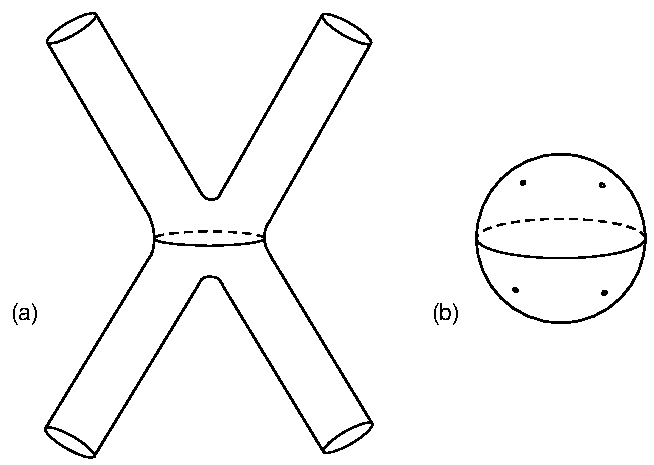
\includegraphics[width=0.8\linewidth]{figures/fig_3_8.pdf}
\caption{(a) 源が $X^0=\pm\infty$ に近づく、四本の閉弦の散乱。(b) 四本の閉弦の散乱を表す共形的に等価な描像。小さな穴をもつ球面となる。}
\label{fig:3.8}
\end{figure}

第2章から知っているように、円筒は座標 $z$ によって共形的に等価に記述できる。
\begin{equation}
z=\exp(-iw),\qquad \exp(-2\pi t)\leq|z|\leq1.
\tag{3.5.2}\label{eq:3.5.2}
\end{equation}
この描像では、長い円筒が単位円板に写され、外部の弦状態は中心にある小さな円になる。内部計量の幾何では、図\hyperref[fig:3.8]{3.8}(a)の過程は、今や図\hyperref[fig:3.8]{3.8}(b)のように見える。$t\to\infty$ の極限では、小さな円は点へ縮み、世界面は、外部状態ごとに一点の挿入をもつ球面に帰着する。

同じ考えは、外部の開弦状態にも成り立つ。図\hyperref[fig:3.9]{3.9}(a)の過程における長い帯は、領域
\begin{equation}
-2\pi t\leq\operatorname{Im}w\leq0,\qquad
0\leq\operatorname{Re}w\leq\pi
\tag{3.5.3}\label{eq:3.5.3}
\end{equation}
として記述できる。$\operatorname{Im}w=-2\pi t$ が源であり、$\operatorname{Re}w=0,\pi$ は弦の端点の境界である。$z=-\exp(-iw)$ の下で、これは単位円板と上半平面の共通部分から、原点の小さな半円を切り取ったものに写る。
\begin{equation}
\exp(-2\pi t)\leq|z|\leq1,\qquad \operatorname{Im}z\geq0.
\tag{3.5.4}\label{eq:3.5.4}
\end{equation}
散乱過程は、今や図\hyperref[fig:3.9]{3.9}(b)のように見える。$t\to\infty$ の極限では、源は（弦の端点の）境界上の点へ縮む。

\begin{figure}[htbp]
\centering
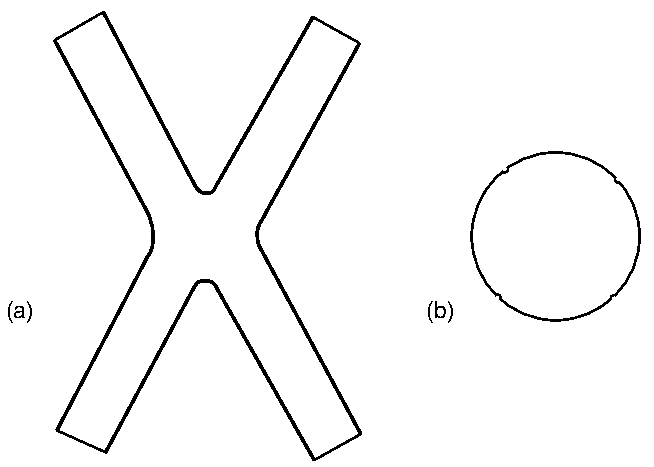
\includegraphics[width=0.8\linewidth]{figures/fig_3_9.pdf}
\caption{(a) 源が $X^0=\pm\infty$ に近づく、四本の開弦の散乱。(b) 共形的に等価な描像。小さなくぼみをもつ円板となる。}
\label{fig:3.9}
\end{figure}

これは、すでに見た状態・演算子対応である。各弦の源は、世界面上の局所的な擾乱となる。$D$ 元運動量 $k^\mu$ と内部状態 $j$ をもつ、与えられた入射または出射の弦には、この極限操作によって決まる局所的な頂点演算子 $\mathcal V_j(k)$ が対応する。入射状態と出射状態は $k^0$ の符号によって区別され、入射状態では $k^\mu=(E,\mathbf k)$、出射状態では $k^\mu=-(E,\mathbf k)$ である。図\hyperref[fig:3.8]{3.8}と\hyperref[fig:3.9]{3.9}は最低次の振幅だけを描いているが、この構成が一般的であることは明らかである。無限遠に伸びる管をもたず、その代わりに、各外部閉弦に対して内部に一点の挿入を、各外部開弦に対して境界上に一点の挿入をもつ、コンパクトな世界面に注意を限ることができる。すると、$n$ 粒子の $S$ 行列要素は
\begin{equation}
\begin{aligned}
S_{j_1\cdots j_n}(k_1,\ldots,k_n)
={}&\sum_{\substack{\text{コンパクトな}\\\text{位相型}}}
\int\frac{[dX\,dg]}{V_{\mathrm{diff}\times\mathrm{Weyl}}}
\exp(-S_X-\lambda\chi)\\
&\quad\times\prod_{i=1}^n
\int d^2\sigma_i\,g(\sigma_i)^{1/2}
\mathcal V_{j_i}(k_i,\sigma_i)
\end{aligned}
\tag{3.5.5}\label{eq:3.5.5}
\end{equation}
によって与えられる。頂点演算子の挿入を微分同相不変にするため、世界面上でそれらを積分した。第1巻の残りでは、この推測が正しく、これが実際に意味のある弦の $S$ 行列を定義することを見るであろう。

四種類の弦理論のうちどれを考えるかに応じて、位相型についての和には、向き付けのない世界面や、境界をもつ世界面、あるいはその両方が含まれる。一般に、位相型についての和は連結な世界面だけに制限されない。全過程には、互いに遠く離れた二組以上の粒子群が独立に散乱する過程が含まれうる。和を連結な曲面に制限して得られる、連結な $S$ 行列に注目すると便利である。

したがって、連結な $S$ 行列を得るには、世界面のコンパクトで連結なすべての位相型について和をとらねばならない。二次元では、そのような位相型の分類はよく知られている。境界をもたない、コンパクトで連結かつ向き付けられた任意の二次元曲面は、$g$ 個の取っ手を付けた球面と位相的に同値である。$g$ は曲面の種数と呼ばれる。図\hyperref[fig:3.10]{3.10}に $g=0,1,2$ を示す。閉曲面に穴を開ければ、境界を加えられる。コンパクトで連結かつ向き付けられた任意の二次元曲面は、$g$ 個の取っ手と $b$ 個の穴をもつ球面に位相的に同値である。たとえば、$(g,b)=(0,1)$ は円板、$(0,2)$ は円環、$(0,3)$ はズボン型曲面である。

\begin{figure}[htbp]
\centering
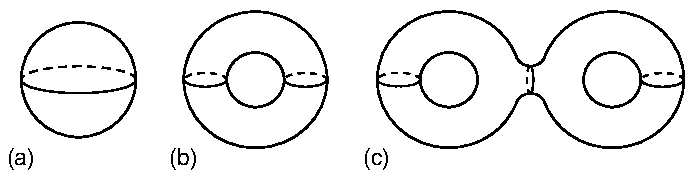
\includegraphics[width=0.8\linewidth]{figures/fig_3_10.pdf}
\caption{種数が (a) 0、(b) 1、(c) 2 の、コンパクトで連結かつ向き付けられた閉曲面。}
\label{fig:3.10}
\end{figure}

向き付けのない曲面を記述するには、クロスキャップを導入すると便利である。曲面に穴を開け、直径の両端にある点を同一視するのである。より詳しくは、複素座標 $z$ をとり、半径が1よりわずかに小さい円板を切り取り、$z'=-1/\bar z$ を満たす点の対を等価と定義することによって、向かい合う点を貼り合わせる。貼り合わせが反正則なので、得られる曲面は向き付けをもたない。また、境界の場合と違って、クロスキャップは縁などの局所的な特徴を導入しない。切り取ることで導入された縁は、単に座標パッチの境界である。向き付けの有無を問わず、コンパクトで連結な任意の閉曲面は、球面に $g$ 個の取っ手と $c$ 個のクロスキャップを加えることで得られる。コンパクトで連結な任意の曲面は、球面に $g$ 個の取っ手、$b$ 個の境界、$c$ 個のクロスキャップを加えることで得られる。実際には、この記述にはいくらか冗長性がある。境界がある場合もない場合も、$g$ と $c$ の両方が同時にゼロでない値をとらないように和を制限すれば、すべての位相型をちょうど一度ずつ得る。たとえば、$(g,b,c)=(0,0,1)$ は射影平面、$(g,b,c)=(0,1,1)$ は Möbius の帯、$(g,b,c)=(0,0,2)$ は Klein の壺である。また、クロスキャップを付けたトーラスは、二つのクロスキャップを一つの取っ手に置き換えることにより、$(g,b,c)=(0,0,3)$ としても $(g,b,c)=(1,0,1)$ としても得られる。Euler 数は
\begin{equation}
\chi=2-2g-b-c
\tag{3.5.6}\label{eq:3.5.6}
\end{equation}
で与えられる。

異なる位相型の数は、場の理論の一定の次数における異なる Feynman 図の数に比べて非常に少ない。たとえば、向き付けられた閉弦の理論では、摂動論の各次数に位相型がちょうど一つ存在する。場の理論では、図の数は次数に対して階乗的に増える。一つの弦の図には、場の理論のすべての図が含まれている。取っ手がその周長に比べて長くなるさまざまな極限では、取っ手を線で近似でき、その極限の弦の図は、対応する Feynman 図で近似される。
